\section{Class 11 - 31/03/21}
Today we are introducing the concept of using multiple antennas to send EM signals. The main advantage of using a cluster of antennas is that we can easily change the radiation pattern without using moving parts, this will let us serve multiple directions with the same antenna geometry.
\subsection*{Two dipole array}
What does happen if we put two dipole antennas at a distance $l$ like in \cref{fig:Two_dipole_array_example}?
\tdplotsetmaincoords{60}{110}
\begin{figure}[H]
    \begin{center}
        \begin{tikzpicture}[scale=5,tdplot_main_coords]
            \pgfmathsetmacro{\rvec}{1.2}
            \pgfmathsetmacro{\thetavec}{45}
            \pgfmathsetmacro{\phivec}{70}
            \coordinate (O) at (0,0,0);
            
            \draw[thick,->] (0,0,0) -- (1,0,0) node[anchor=north east]{$x$};
            \draw[thick,->] (0,0,0) -- (0,1,0) node[anchor=north west]{$y$};
            \draw[thick,->] (0,0,0) -- (0,0,1) node[anchor=south]{$z$};
            \draw[dashed] (0,0,0) -- (0,0,-0.3);

            \tdplotsetrotatedcoords{0}{0}{20}

            \draw[line width=0.7mm,tdplot_rotated_coords, color=blue!50!black]  (0,0.03,0.25) -- (0,0.2,0.25) node[above]{d1};
            \draw[line width=0.7mm,tdplot_rotated_coords, color=blue!50!black] (0,-0.03,0.25) -- (0,-0.2,0.25);

            \draw[line width=0.7mm,tdplot_rotated_coords, color=blue!50!black]  (0,0.03,-0.25) -- (0,0.2,-0.25) node[above]{d2};
            \draw[line width=0.7mm,tdplot_rotated_coords, color=blue!50!black] (0,-0.03,-0.25) -- (0,-0.2,-0.25);

            \draw [decorate,decoration={brace,amplitude=6pt,mirror},tdplot_rotated_coords]
            (0,-0.22,0.25) -- (0,-0.22,-0.25) node[midway,left,xshift=-1ex]{$l$};

            \tdplotsetcoord{P}{\rvec}{\thetavec}{\phivec}
            \tdplotsetcoord{P2}{\rvec +0.2}{\thetavec}{\phivec}
            \draw[dotted,tdplot_rotated_coords] (0,0,0.25) -- (P);
            \draw[dotted,tdplot_rotated_coords] (0,0,-0.25) -- (P);

            \draw[-stealth,color=red!80!black,tdplot_rotated_coords] (P) -- (P2) node[above right] {$\overline{E}(r,\varphi,\theta)$};

        \end{tikzpicture}
    \end{center} \caption{Two dipole array example}\label{fig:Two_dipole_array_example} 
\end{figure}
From \cref{eq:electric_field_antenna1}, and assuming the equivalent momentum to be $M=I_0\,d$ (true for the hertzian dipole in far field) we can write the electric field generated by a dipole:
\begin{equation}\label{eq:electric_field_antenna_hertzian}
    \overline{E}(\theta,\varphi)=j\eta\frac{I_0\,d}{2\lambda}\sin(\theta)\,\frac{e^{\,-jkr}}{r}
\end{equation}
From the example in \cref{fig:Two_dipole_array_example} we can see that the antenna are rotated by $90\si{\degree}$, so \cref{eq:electric_field_antenna_hertzian} becomes:
\begin{equation}\label{eq:electric_field_antenna_hertzian_rotated}
    \overline{E}(\theta,\varphi)=j\eta\frac{I_0\,d}{2\lambda}\cos(\theta)\,\frac{e^{\,-jkr}}{r}
\end{equation}
Then we want to find the value of the total electric field $E_T$ on far field region. The equation of $E_T$ should look like this:
\begin{align}\label{eq:electric_field_dual_array1}
    \begin{split}
    \overline{E_T}(\theta,\varphi)&=\overline{E_1}(\theta,\varphi)+\overline{E_2}(\theta,\varphi)=\\[5pt]
    &=j\eta\frac{I_0\,d}{2\lambda}\left( \cos(\theta_1)\,\frac{e^{\,-jkr_1}}{r_1}\,e^{-j\frac{\delta}{2}}+ \cos(\theta_2)\,\frac{e^{\,-jkr_2}}{r_2}\,e^{j\frac{\delta}{2}} \right)
    \end{split}
\end{align}
The equation is simply the sum of the two electric field, and $\delta$ is the phase difference between the current feeding the two dipoles. It does mean that we have full control on it, and we will see that it will be a very interesting parameter.\\
In \cref{fig:Two_dipole_array_example_angle} you can see an example of electric field generated by an array of two dipoles

\begin{figure}[H]
    \begin{center}
        \begin{tikzpicture}[scale=5,tdplot_main_coords]
            \pgfmathsetmacro{\rvec}{1.2}
            \pgfmathsetmacro{\thetavec}{45}
            \pgfmathsetmacro{\phivec}{70}
            \coordinate (O) at (0,0,0);
            
            \draw[thick,->] (0,0,0) -- (1,0,0) node[anchor=north east]{$x$};
            \draw[thick,->] (0,0,0) -- (0,1,0) node[anchor=north west]{$y$};
            \draw[thick,->] (0,0,0) -- (0,0,1) node[anchor=south]{$z$};
            \draw[dashed] (0,0,0) -- (0,0,-0.3);

            \tdplotsetrotatedcoords{0}{0}{20}

            \path[draw=black,fill=black] (0,0,0.25) circle (0.01cm) ;
            \path[draw=black,fill=black] (0,0,-0.25) circle (0.01cm) ;

            \tdplotsetcoord{P}{\rvec}{\thetavec}{\phivec}
            \tdplotsetcoord{P2}{\rvec +0.2}{\thetavec}{\phivec}
            \draw[dotted,tdplot_rotated_coords] (0,0,0.25) -- (P) node[midway,yshift=-7pt]{$r_1$};
            \draw[dotted,tdplot_rotated_coords] (0,0,-0.25) -- (P)node[midway,yshift=-10pt]{$r_2$};

            \draw[-stealth,color=red!80!black,tdplot_rotated_coords] (P) -- (P2) node[above right] {$\overline{E}(r,\varphi,\theta)$};

            \tdplotsetthetaplanecoords{\phivec-50+90}
            \tdplotdrawarc[tdplot_rotated_coords,->]{(0,0,0.35)}{0.2}{0}%
                {\thetavec+5}{anchor=south west}{$\theta_1$}
                \tdplotdrawarc[tdplot_rotated_coords,->]{(0,0,-0.45)}{0.2}{0}%
                {\thetavec-10}{anchor=south west,fill=white,text opacity=1,fill opacity=0.6}{$\theta_2$}

        \end{tikzpicture}
    \end{center} \caption{Electric field generated by two dipoles}\label{fig:Two_dipole_array_example_angle} 
\end{figure}
From what the example on \cref{fig:Two_dipole_array_example_angle} we can make some assumptions: we said that we are in far field condition, so $r_1\approx r_2\approx r$, and this mean that the two angles are equal $\theta_1\approx\theta_2$\\
We will write again the \cref{eq:electric_field_dual_array1}, by assuming $\theta_1\approx\theta_2\approx\theta$, but keeping the two distances separated ($r_1\neq r_2$):
\begin{equation}\label{eq:electric_field_dual_array2}
    E_T=j\eta\frac{I_0\,d}{2\lambda}\frac{\cos(\theta)}{r}\left\{e^{\,-jkr_1}e^{\,-j\frac{\delta}{2}}+e^{\,-jkr_2}e^{\,j\frac{\delta}{2}}\right\}
\end{equation}
In \cref{fig:Two_dipole_array_example_far_field} a sketch of the situation that we are working with.
\begin{figure}[H]
    \begin{center}
        \begin{tikzpicture}[scale=5,tdplot_main_coords]
            \pgfmathsetmacro{\rvec}{1.2}
            \pgfmathsetmacro{\thetavec}{45}
            \pgfmathsetmacro{\phivec}{70}
            \coordinate (O) at (0,0,0);
            
            \draw[thick,->] (0,0,0) -- (1,0,0) node[anchor=north east]{$x$};
            \draw[thick,->] (0,0,0) -- (0,1,0) node[anchor=north west]{$y$};
            \draw[thick,->] (0,0,0) -- (0,0,1) node[anchor=south]{$z$};
            \draw[dashed] (0,0,0) -- (0,0,-0.3);

            \tdplotsetrotatedcoords{0}{0}{20}

            \path[draw=black,fill=black] (0,0,0.25) circle (0.01cm) ;
            \path[draw=black,fill=black] (0,0,-0.25) circle (0.01cm) ;

            \tdplotsetcoord{P0}{\rvec}{\thetavec}{\phivec}
            \tdplotsetcoord{P1}{\rvec}{\thetavec}{\phivec+10}
            \tdplotsetcoord{P2}{\rvec}{\thetavec}{\phivec-10}

            \draw [decorate,decoration={brace,amplitude=6pt,mirror},tdplot_rotated_coords]
            (0,-0.06,0.25) -- (0,-0.06,-0.25) node[midway,left,xshift=-1ex]{$l$};

            %directions of E
            \draw[dotted,tdplot_rotated_coords] (0,0,-0.25) -- (0,1.9,0.9-0.25) node[midway,yshift=6pt]{$r_2$};
            \draw[dotted,tdplot_rotated_coords] (0,0,0.25) -- (0,1.9,0.9+0.25) node[midway,yshift=6pt]{$r_1$};
            \draw[dotted,tdplot_rotated_coords] (0,0,0) -- (0,1.9,0.9) node[midway,yshift=6pt]{$r$};
            %dotted little segment
            \draw[dotted,tdplot_rotated_coords] (0,0,0.25) -- (0,0.1,0.03);
            \draw[dotted,tdplot_rotated_coords] (0,0,0) -- (0,0.1,0.03-0.25);
            %
            \draw[thick,tdplot_rotated_coords,red!50!black] (0,0,0) -- (0,2/21,0.9/21) node[below,fill=white,text opacity=1,fill opacity=0.6,outer sep=0pt,inner sep=0pt,yshift=-2pt,rounded corners=2pt]{\scriptsize{$\Delta r_0$}};
            %\draw[thick,tdplot_rotated_coords,red!50!black] (0,0,0.25) -- (0,2/21,0.9/21+0.25) node[below,fill=white,text opacity=1,fill opacity=0.6,outer sep=0pt,inner sep=0pt,yshift=-2pt,rounded corners=2pt]{\scriptsize{$\Delta r_1$}};
            \draw[thick,tdplot_rotated_coords,red!50!black] (0,0,-0.25) -- (0,2/21,0.9/21-0.25) node[below,fill=white,text opacity=1,fill opacity=0.6,outer sep=0pt,inner sep=0pt,yshift=-2pt,rounded corners=2pt]{\scriptsize{$\Delta r_2$}};
            \tdplotsetthetaplanecoords{\phivec-50+90}
            \tdplotdrawarc[tdplot_rotated_coords,->]{(0,0,0.35)}{0.2}{0}%
                {\thetavec}{anchor=south west}{$\theta$}

            
        \end{tikzpicture}
    \end{center} \caption{Two dipole array electric field direction in far field condition}\label{fig:Two_dipole_array_example_far_field} 
\end{figure}
You can notice that with all the assumptions we have made, it is easy to find the distance of the electric $r$ field from the two dipoles by looking at the two segments $\Delta r_0$ and $\Delta r_2$.\\
we know that:
\begin{center}
    \begin{tabular}{ c c c }
        $\Delta r_0=r_1-r$&
        and&
        $\Delta r_2=r-r_2$
    \end{tabular}
\end{center}
And with some trigonometry, by noticing that $\theta$ is equal for all the segments we can say that a segment can be seen as $\text{segment}=\frac{l\,\cos(\theta)}{2}$, so:
\begin{center}
    \begin{tabular}{ c c c }
        $r_1=r-\frac{l}{2}\cos(\theta)$&
        and&
        $r_2=r+\frac{l}{2}\cos(\theta)$
    \end{tabular}
\end{center}
Then \cref{eq:electric_field_dual_array2} will become:
\begin{align}
    \begin{split}
        E_T&=j\eta\frac{I_0\,d}{2\lambda}\frac{\cos(\theta)}{r}\left\{e^{\,-jk(r-\frac{l}{2}\cos(\theta))}e^{\,-j\frac{\delta}{2}}+e^{\,-jk(r-\frac{l}{2}\cos(\theta))}e^{\,j\frac{\delta}{2}}\right\}\\[5pt]
        &=j\eta\frac{I_0\,d}{2\lambda}\,\cos(\theta)\,\frac{e^{\,-jkr}}{r}\left\{e^{\,j(k\frac{l}{2}\cos(\theta)-\frac{\delta}{2})}+e^{\,-j(k\frac{l}{2}\cos(\theta)-\frac{\delta}{2})}\right\}\\[5pt]
    \end{split}
\end{align}
We could see the last part of exponentials as:
\begin{equation}
    e^{\,j\alpha}+e^{\,-j\alpha}=\frac{e^{\,j\alpha}+e^{\,-j\alpha}}{2}\cdot 2=2\,\cos(\alpha)    
\end{equation}
Then we obtain the final expression of the total electric field:
\begin{equation}\label{eq:electric_field_dual_array3}
    E_T=\underbrace{j\eta\frac{I_0\,d}{2\lambda}\,\cos(\theta)\,\frac{e^{\,-jkr}}{r}}_{\text{Single dipole eq.}}\;\cdot\;\underbrace{2\cos\left(\frac{1}{2}(k\,l\,\cos(\theta)-\delta)\right)}_{\text{Array factor}}
\end{equation}
The expression of $E_T$ in \cref{eq:electric_field_dual_array2} can be seen as the combination of two parts: the first one is the expression of $E$ for the hertzian dipole that we have already seen in \cref{eq:EMF_components_in_spherical_2}, ant the second one is the expression of how the total field changes depending on $l$, $\theta$ and $\delta$.\\
This second part of the $E_T$ equation is usually called \emph{Array Factor} $AF$, so the \cref{eq:electric_field_dual_array3} could be seen as:
\begin{equation}
    E_T=\text{Dipole eq.} \cdot AF
\end{equation}
and in a more general form:
\begin{equation}
    E_T=\text{Antenna eq.} \cdot AF
\end{equation}
This expression is very good, because we can study complex antenna arrays by multiplying the equation of one of the antenna array, with the AF.
\subsubsection*{Example of array patterns with hertzian dipole}
In this example we will see an antenna array composed by two hertzian dipoles.\\
First of all, we look back at the radiation pattern of the hertzian dipole in \cref{fig:Dipolexz}, and we rotate it by $90\si{\degree}$. Then we will multiply it by the Array Factor.
\begin{figure}[H]
    \begin{center}
        \resizebox{0.45\textwidth}{!}{%
        \begin{tikzpicture}
            \begin{polaraxis}[axis lines = none]
                \addplot[domain=0:360,samples=73,smooth] (x+90,{abs(cos(x))});
            \end{polaraxis}
            \draw[-stealth] ([yshift=-0.5cm]current axis.south) -- ([yshift=0.5cm]current axis.north) node[anchor=north,xshift=4pt]{$z$};
            \draw[-stealth] (current axis.west) -- (current axis.east) node[anchor=west]{$x$};
        \end{tikzpicture}}
        \caption{Hertzian dipole rotated by $90\si{\degree}$}\label{fig:Dipolexyrotated}
    \end{center}
\end{figure}
In order to find the array factor pattern, we will evaluate $AF$ for different $\theta$ value, in this way we can multiply $I_r\cdot AF$ to find the total radiation pattern.\\
Why we are multiplying the radiation pattern and not the electric field? Because $I_r$ is very much related to $E$, as we have seen in \cref{eq:radiation_intensity}.\\
Note that also $AF$ related to the radiation pattern does change a bit, but we will give some "graphical" intuition, not the real mathematical expression.
\subsubsection*{Case $\theta=0$}
First of all we need to consider
\begin{itemize}
    \item $\bm{L=\frac{\lambda}{4}}$
    \item $\bm{\delta=\frac{\pi}{2}}$
\end{itemize}
If $\theta=0$, then the array factor will become:
\begin{equation}
    AF=2\cos\left\{\frac{1}{2}\left(\frac{2\pi}{\lambda}\,\frac{\lambda}{4}-\frac{\pi}{2}\right)\right\}=2\cos(0)=2
\end{equation}
So for $\theta=0$ the array factor is the maximum
\subsubsection*{Case $\theta=\pi$}
The array factor in this case will be:
\begin{equation}
    AF=\cos\left(\frac{\pi}{4}-\frac{\pi}{2}\right)=0
\end{equation}
So, for $\theta=\pi$ the array factor is the minimum possible ($AF=0$)
\subsubsection*{We continue trying different $\theta$ values...}
If we continue to move $\theta$ around, we will obtain the full pattern of the $AF$.
\begin{figure}[H]
    \begin{center}
        \begin{tikzpicture}
            \begin{polaraxis}[axis lines = none]
                \addplot[domain=0:360,samples=73,smooth] (x+270,{3-(3*cos(x))});
            \end{polaraxis}
            \draw[-stealth] ([yshift=3cm]current axis.south) -- ([yshift=0.5cm]current axis.north) node[anchor=north,xshift=4pt]{$z$};
            \draw[-stealth] (current axis.west) -- (current axis.east) node[anchor=west]{$x$};
        \end{tikzpicture}
        \caption{Antenna Factor pattern for dual array dipole}\label{fig:AFhertzian}
    \end{center}
\end{figure}
At the end, if we multiply the radiation pattern in \cref{fig:Dipolexyrotated}, and the $AF$ pattern in \cref{fig:AFhertzian}, you will obtain the total radiation pattern of the array of hertzian dipole.
\begin{figure}[H]
    \begin{center}
        \begin{tikzpicture}
            \begin{polaraxis}[axis lines = none]
                \addplot[domain=0:360,samples=73,smooth] (x+270,{(3-(3*cos(x)))*abs(cos(x))});
            \end{polaraxis}
            \draw[-stealth] ([yshift=3cm]current axis.south) -- ([yshift=0.5cm]current axis.north) node[anchor=north,xshift=4pt]{$z$};
            \draw[-stealth] (current axis.west) -- (current axis.east) node[anchor=west]{$x$};
        \end{tikzpicture}
        \caption{Total radiation pattern of the dual array of hertzian dipoles}\label{fig:tot_radiation_array}
    \end{center}
\end{figure}
\subsubsection*{What if I change the phase?}
If we change the phase, we control the direction of the pattern, this mean that we change the radiation pattern without having moving parts.
\subsection*{Symmetries on fields}
Sometimes we can use the symmetries of the domain with respect to the $X\,Y$ plane to obtain some interesting properties.
\subsubsection*{Even symmetry}
If a field has an even symmetry with respect to the $X\,Y$ plane, we can say that it is \emph{Even symmetric}(\cref{fig:even_sym}), and his electric field could be described by:
\begin{align}
    \begin{split}
        E_x(x,y,z)&=E_x(x,y,-z)\\[5pt]
        E_y(x,y,z)&=E_y(x,y,-z)\\[5pt]
        E_z(x,y,z)&=-E_z(x,y,-z)\\[5pt]
    \end{split}
\end{align}
\begin{figure}[H]
    \begin{center}
        \resizebox{0.5\textwidth}{!}{%
            \begin{tikzpicture}[declare function={f(\x,\y)=2*\x*\y;},scale=2.5]
                \def\xmax{1} \def\xmin{-1.2}
                \def\ymax{1} \def\ymin{-1.2}
                \def\nx{15}  \def\ny{15}
                
                \pgfmathsetmacro{\hx}{(\xmax-\xmin)/\nx}
                \pgfmathsetmacro{\hy}{(\ymax-\ymin)/\ny}
                \foreach \i in {0,...,\nx}
                \foreach \j in {0,...,\ny}{
                \pgfmathsetmacro{\yprime}{f({\xmin+\i*\hx},{\ymin+\j*\hy})}
                \draw[teal,-stealth,shift={({\xmin+\i*\hx},{\ymin+\j*\hy})}] 
                (0,0)--($(0,0)!1mm!(.1,.1*\yprime)$);
                }
                
                \draw[-stealth] (\xmin-0.2,0) -- (\xmax+0.2,0) node[anchor=north,xshift=4pt]{$x$};
                \draw[-stealth] (\xmin-0.1,\ymin-0.1) -- (\xmin-0.1,\ymax+0.2) node[anchor=north,xshift=4pt]{$z$};
             
            \end{tikzpicture}}
        \caption{Even symmetry}\label{fig:even_sym} 
    \end{center}
\end{figure}
\subsubsection*{Odd symmetry}
In the \emph{Odd symmetry}(\cref{fig:odd_simmetry}) the electric field could be described as:
\begin{align}
    \begin{split}
        E_x(x,y,z)&=-E_x(x,y,-z)\\[5pt]
        E_y(x,y,z)&=-E_y(x,y,-z)\\[5pt]
        E_z(x,y,z)&=\;E_z(x,y,-z)\\[5pt]
    \end{split}
\end{align}
\begin{figure}[H]
    \begin{center}
    \resizebox{0.5\textwidth}{!}{%
    \begin{tikzpicture}[declare function={f(\x,\y)=0.5/\y;},scale=2.5]
        \def\xmax{1} \def\xmin{-1.2}
        \def\ymax{1} \def\ymin{-1.2}
        \def\nx{15}  \def\ny{15}
        
        \pgfmathsetmacro{\hx}{(\xmax-\xmin)/\nx}
        \pgfmathsetmacro{\hy}{(\ymax-\ymin)/\ny}
        \foreach \i in {0,...,\nx}{
        \foreach \j in {9,...,15}{
        \pgfmathsetmacro{\yprime}{f({(\xmin+\i*\hx)},{\ymin+\j*\hy})}
        \draw[teal,-stealth,shift={({\xmin+\i*\hx},{\ymin+\j*\hy})}] 
        (0,0)--($(0,0)!1mm!(.1,.1*\yprime)$);
        }
        \foreach \k in {0,...,8}{
        \pgfmathsetmacro{\yprime}{f({(\xmin+\i*\hx)},{abs(\ymin+\k*\hy)})}
        \draw[teal,-stealth,shift={({\xmin+\i*\hx},{\ymin+\k*\hy})}] 
        (0,0)--($(0,0)!1mm!(-.1,.1*\yprime)$);
        }
        }
        
        
        %axes
        \draw[-stealth] (\xmin-0.2,0) -- (\xmax+0.2,0) node[anchor=north,xshift=4pt]{$x$};
        \draw[-stealth] (\xmin-0.1,\ymin-0.1) -- (\xmin-0.1,\ymax+0.2) node[anchor=north,xshift=4pt]{$z$};
    \end{tikzpicture}}
    \end{center}\caption{Odd symmetry}\label{fig:odd_simmetry} 
\end{figure}
This odd symmetry is interesting: by his definition, when the electric field approach the $X\,Y$ plane the $E_x$ component reduces, until it touches the symmetry plane where it becomes $E_x=0$.\\
Does it sound familiar to you? it is the definition of the electric field reflecting to the metallic surface!\\
So, whenever I have my antenna transmitting near a metallic surface, I could study it by considering the metal as an odd symmetry plane, this will simplify a lot the study and the computation needed to inspect the electric field in that case (because I am calculating only half of the circuit).\\
What about a magnetic boundary? They does not exist in nature, but we can exploit this symmetry property in some particular cases to simplify the computation.
\subsubsection*{Case study with symmetry}
The odd symmetry property could be an useful case study also in real life!
Let's consider the tv broadcast antenna that you can find in the roof of every house, it is a very omnidirectional antenna, and sometimes to increase its directivity we could add a metallic grid in order to channeling the radiation into the dipole (that is the sensitive part of the antenna).\\
We consider for simplicity an antenna with only one dipole, as shown in a simplified representation in \cref{fig:shielded_dipole}
\begin{figure}[H]
    \begin{center}
        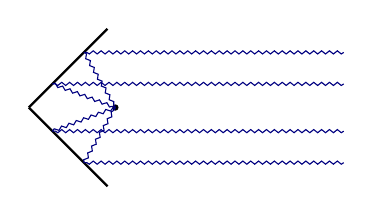
\begin{tikzpicture}[%
            wave/.style={%
              -,
              %shorten >=4pt,
              %shorten <=4pt,
              decorate,
              decoration={%
                snake,
                segment length=1mm,
                amplitude=0.2mm,
                pre length=0pt,
                 post length=0pt,
              }
            }
          ]
            %antenna 1
            \fill [black] (1.1,0) circle (0.4mm);
            \draw [black,thick] (0,0) -- (1,1);
            \draw [black,thick] (0,0) -- (1,-1);
            %radiation
            \draw [blue!50!black,wave,-,decorate] (4,0.7) -- (0.7,0.7);
            \draw [blue!50!black,wave,-,decorate] (0.7,0.7) -- (1.1,0);

            \draw [blue!50!black,wave,-,decorate] (4,-0.7) -- (0.7,-0.7);
            \draw [blue!50!black,wave,-,decorate] (0.7,-0.7) -- (1.1,0);

            \draw [blue!50!black,wave,-,decorate] (4,0.3) -- (0.3,0.3);
            \draw [blue!50!black,wave,-,decorate] (0.3,0.3) -- (1.1,0);

            \draw [blue!50!black,wave,-,decorate] (4,-0.3) -- (0.3,-0.3);
            \draw [blue!50!black,wave,-,decorate] (0.3,-0.3) -- (1.1,0);

          \end{tikzpicture}
    \end{center}\caption{Side view of a shielded dipole antenna}\label{fig:shielded_dipole}
\end{figure}
If you want to investigate the electric field of this type of antenna, the computation would be quite heavy. But we notice that the total electric field is odd symmetric with the two shields: so we have the possibility to study the field $E$ by removing the shields and considering a fictitious antenna array that recreate the symmetry.\\
\textbf{The end.} 